\documentclass[12pt,a4paper]{article}
\usepackage[utf8]{inputenc}
\usepackage[T1]{fontenc}
\usepackage[english]{babel}
\usepackage{fancyhdr}
\usepackage{kpfonts}
\usepackage[margin=1in]{geometry}
\usepackage{exsheets}
\usepackage{amsmath, amssymb, amsfonts}
\usepackage{enumerate}
\usepackage{tikz}
\usepackage{tabularx}
\usetikzlibrary{arrows, decorations.text}

\pagestyle{fancy}
\renewcommand{\headrulewidth}{2pt}
\fancyhead[L]{EPITA\_ING1\_BING\_2021\_S6\_PARTIEL\_GREF}
\fancyhead[R]{April 2019}

\fancyfoot[C]{\textbf{\thepage}}
\fancyfoot[L]{}

\SetupExSheets{solution/print=true}
\SetupExSheets{question/type=exam}
\SetupExSheets[points]{name=point,name-plural=points}
\RenewQuSolPair{question}[name={\large Exercise}]{solution}

\begin{document}
\begin{center}

  {\Large \textbf{Networks and Flows on Graphs\footnote{Head of course : P.~Siarry.}}}\\

  \vspace{10pt}
  {\Large \textit{Final Exam}}

  \vspace{2\baselineskip}
\end{center}
\begin{center}
\begin{minipage}{\textwidth}
  Duration of the exam : 1h30\\
  No documents are allowed\\
  Only \emph{non-programmable} pocket calculators are allowed\\
  Exercises can be done independently.
\end{minipage}
\end{center}
\rule{\textwidth}{2pt}

\vspace{\baselineskip}

\begin{question}
  Using Floyd-Warshall's algorithm, compute all minimal paths between
  any two pairs of vertices of the following graph. Could we look for
  all maximal paths between any such pairs?  \vspace{2\baselineskip}
  \begin{center}
    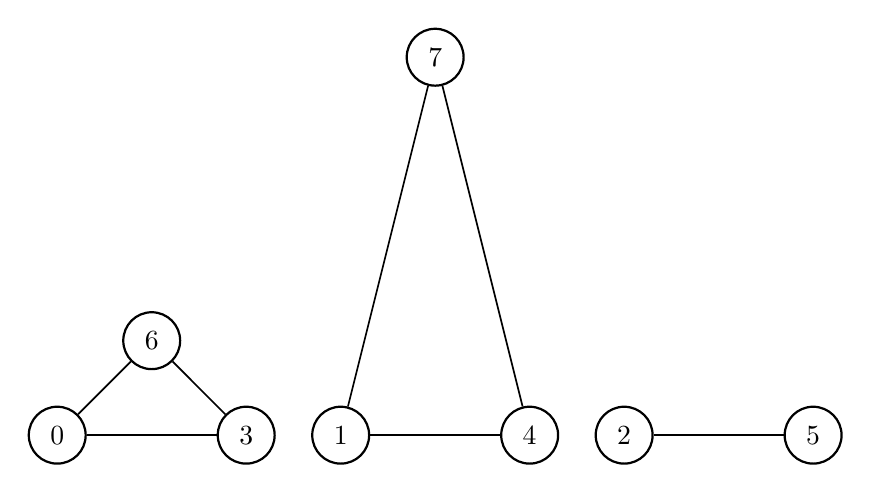
\begin{tikzpicture}
      [minimum width={width("b")+1.5em},
      vertex/.style={circle, draw=black, fill=white, thick},
      arr/.style={-,semithick},
      scale=1.2]
      \node (0) at (0, 0) [vertex] {$0$};
      \node (3) at (2, 0) [vertex] {$3$}
      edge[arr] (0);
      \node (6) at (1, 1) [vertex] {$6$}
      edge[arr] (0)
      edge[arr] (3);
      \node (1) at (3, 0) [vertex] {$1$};
      \node (4) at (5, 0) [vertex] {$4$}
      edge[arr] (1);
      \node (7) at (4, 4) [vertex] {$7$}
      edge[arr] (1)
      edge[arr] (4);
      \node (2) at (6, 0) [vertex] {$2$};
      \node (5) at (8, 0) [vertex] {$5$}
      edge[arr] (2);
    \end{tikzpicture}
  \end{center}
  \vspace{2\baselineskip}
\end{question}

\begin{question}
  A project is described by the following dependancy table
  \begin{center}
    \renewcommand{\arraystretch}{1.5}
    \begin{tabularx}{.825\textwidth}{|c|p{6.75cm}|c|}
      \hline
      Label of task & Requirements before task starts & Time (in days)  \\
      \hline
      A  & & $10$  \\
      \hline
      B  &  & $15$  \\
      \hline
      C  & A finished, B finished since $3$ days & $11$  \\
      \hline
      D  & A finished since $7$ days & $7$  \\
      \hline
      E  & A started since $16$ days, B finished & $9$ \\
      \hline
      F  & B finished since $2$ days & $14$  \\
      \hline
      G  & D finished, C finished since $1$ day & $7$ \\
      \hline
      H  & E finished & $12$ \\
      \hline
      I  & E finished since $6$ days & $8$  \\
      \hline
    \end{tabularx}
  \end{center}
  \vspace{\baselineskip}
  \begin{enumerate}
  \item Draw the MPM (Meta Potential Model) graph of this project
    planning problem.
  \item Using relevant algorithms, give earliest scheduling dates.
    \begin{itemize}
    \item What is the minimum amount of time the project needs to be done?
    \item What are the critical tasks?
    \item Represent project scheduling as a Gantt diagram.
    \end{itemize}
  \item Using relevant algorithms, give latest scheduling dates.
    \begin{itemize}
    \item Compute margins and free margins of non-critical tasks?
    \end{itemize}
  \end{enumerate}
\end{question}

\end{document}

%%% Local Variables:
%%% mode: latex
%%% TeX-master: t
%%% End:
